\documentclass[11pt,a4paper]{article}
\usepackage{graphicx}
\usepackage[cp1250]{inputenc} 
\usepackage[]{units}
\usepackage{textgreek}
\title{Chapman - Jouguet conditions in methane-hydrogen-air mixtures}
\author{Mateusz Klos}
\date{Computational methods in combustion\\
Warsaw University of Technology}

\begin{document}
\maketitle

\clearpage
\tableofcontents
\clearpage
% pierwsza sekcja
\section{Introduction}\label{sec:intro}
This report presents a study of the CJ conditions in various propane - hydrogen - oxygen mixtures. The calculations were performed in SDToolbox, using "wang\_highT" mechanism of kinetics and two functions: "CJSpeed" and "Postshock\_eq".

\section{Mathematical model}\label{sec:model}
The solver is based on the simpliest, 1-dimensional model of detonation, proposed by Chapman and Jouguet around 1900. It treats the detonation wave as a discontinuity in flow, allowing the use of three basic conservation laws: mass, momentum and energy.

\begin{equation}
    \rho_1 w_1 = \rho_2 w_2
\end{equation}
\begin{equation}
    p_1 + \rho_1 w_1 u_1 =p_2 + \rho_2 w_2 u_2
\end{equation}
\begin{equation}
    \frac{1}{2} w_1^2 + \frac{\kappa}{\kappa - 1} \frac{p_1}{\rho_1} = \frac{1}{2} w_2^2 + \frac{\kappa}{\kappa - 1} \frac{p_2}{\rho_2} + H
\end{equation}

Where:\\
$p$ - pressure\\
$\rho$ - density\\
$w$ - velocity of shockwave propagation\\
$u$ - velocity of gas\\
$H$ - heat coming from chemical reaction\\
Index 1 denotes parameters before shockwave, while 2 denotes parameters behind the shockwave.
\\
\\
Knowing H of a given mixture(from Cantera), one can calculate all the other thermodynamic parameters. 



\section{Results}\label{sec:results}
The initial thermodynamic conditions of a mixture are:\\
p = 1 bar\\
T = 300K\\

Five propane concentrations were taken into consideration - 0\%, 3\%, 6\%, 9\% and 12\%. The concentration of hydrogen varies constantly from 5 to 80\%. It was hard to determine the ignition limits for this mixture, so the results are presented for whole spectrum of concentrations.\\
The following plots show three basic parameters of a detonative combustion - CJ speed, pressure and temperature behind the wave.



\begin{figure}[t]
    \centering
    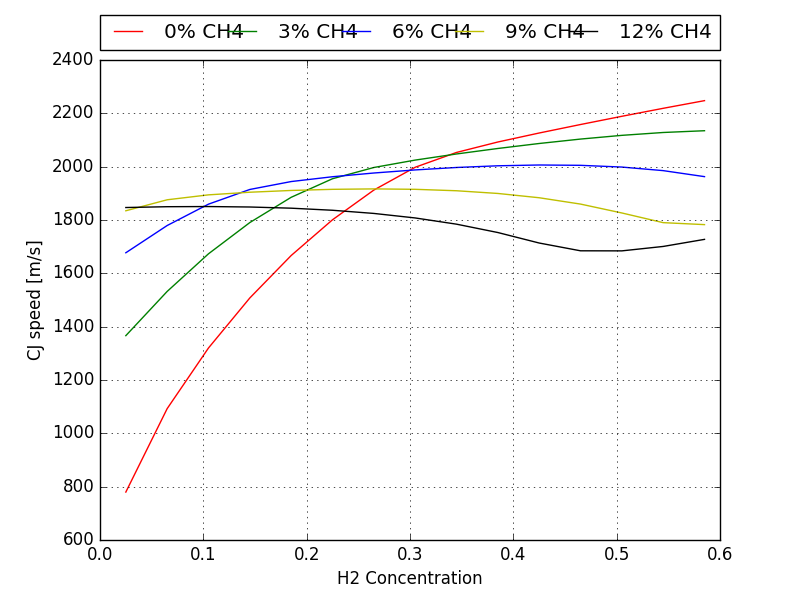
\includegraphics[width=1.2\textwidth]{plot_CJ}
    \caption{.         Chapman Jouguet velocity vs H2 and CH4 concentration}
    \label{fig:CJ}
\end{figure}
What can be read from Fig \ref{fig:CJ} is that there is no maximum CJ speed for a pure hydrogen - air mixture. As the amount of methane increases, the point of maximum moves to the lower hydrogen concentrations.
\begin{figure}[t]
    \centering
    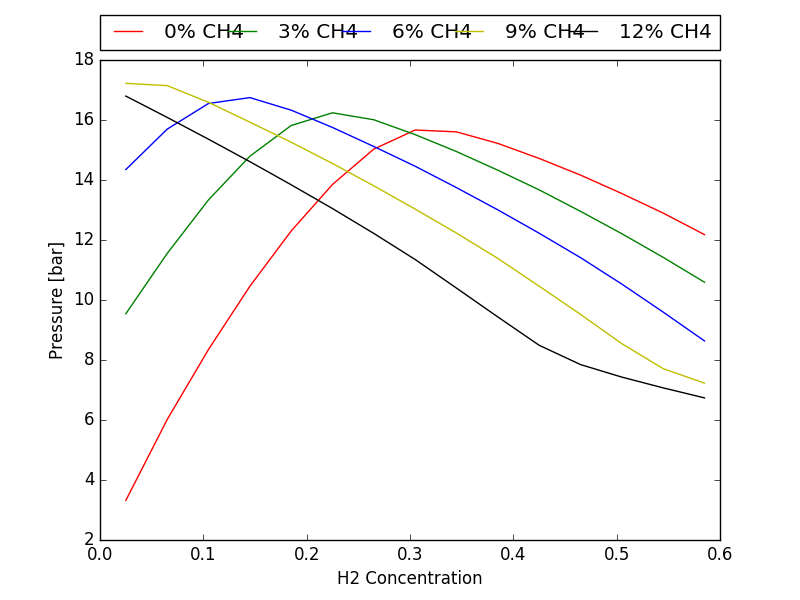
\includegraphics[width=1.2\textwidth]{plot_P}
    \caption{.          Chapman Jouguet pressure vs H2 and CH4 concentration}
    \label{fig:P}
\end{figure}
The chart shows correlation between methane, hydrogen concentration and pressure. For higher methane concentration there is rise in pressure, up to 17.2 bar.
\clearpage
\begin{figure}[t]
    \centering
    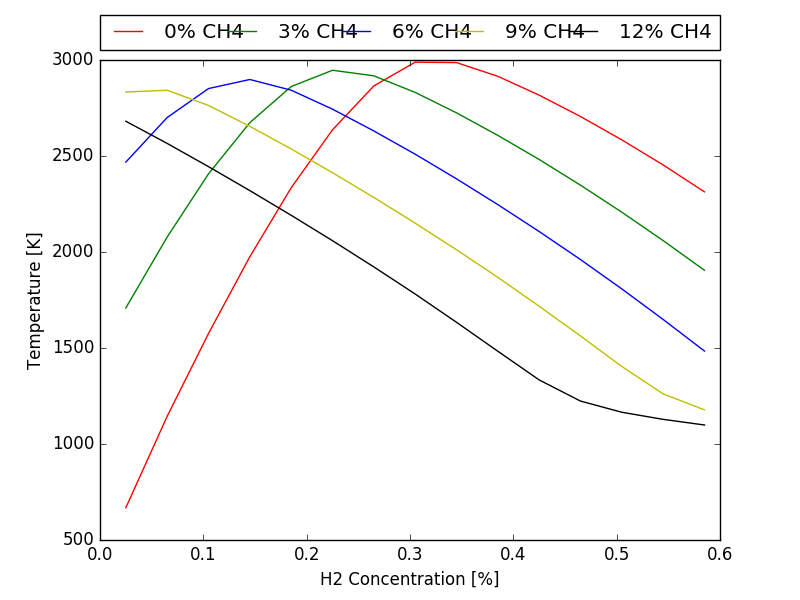
\includegraphics[width=1.2\textwidth]{plot_T}
    \caption{.        Chapman Jouguet temperature vs H2 and CH4 concentration}
    \label{fig:T}
\end{figure}

The chart shows correlation between methane, hydrogen concentration and temperature. For higher methane concentration there is drop in temperature, from 3000K to 2700K.



\section{Summary}\label{sec:summary}
- The CJ speed for pure hydrogen-air mixtures increases with hydrogen concentration\\
- With methane added, the maximum starts to appear\\
- For highest and lowest methane concentration pressure differs 10\%, whilst temperature only 3\%.
- Maximum pressure increases for higher methane concentration and lower hydrogen concentration, whilst maximum temperature increases for lower methane concentration and higher hydrogen concentration.







\end{document}
